documentclass[10.5pt, a4paper]{article}
\usepackage{amsfonts}
\usepackage[top=1in,left=1in,right=1in]{geometry}
\usepackage{times}
\usepackage{tabularx}
\usepackage{graphicx}
\title{Rang de Basanti}
\Author{Romal, Pooja and Saketh}
\begin{document}
\maketitle
\textbf{Title: rang de basanti}

A thought-provoking, soul-stirring wake up call to the youth of India. An engrossing entertainer from a genre
 that's still young in Indian cinema. A film that fiercely eyeballs you, grabs you by the solar and rattles the
 nonchalance out of you. A glorious tapestry with layers upon layers of the moments and decisions that make the
 lives of beautifully defined characters. Engrossing entertainment meets taut social comment with perfect timing
 in Rang De Basanti. Wake up India, Rang De Basanti is here!

Sight & Sound magazine conducts a poll every ten years of the world's finest film directors to find out the Ten Greatest Films of All Time. This poll has been going since 1992, and has become the most recognised[78] poll of its kind in the world. In 2012[79] Cyrus Frisch voted for "Rang De Basanti". Frisch commented: "Corruption became the subject of fierce debate in India after the major success of this film among youngsters."

Rang De Basanti had a noticeable impact on Indian society. A study of bloggers behavioral patterns during the first month of the film's release revealed a significant increase in public ire towards government and politicians for constantly being mired in corruption and bureaucracy and their inefficiency in providing basic amenities. 

In the first half, the film develops these characters and precisely tells the audience how close they unconsciously are to their characters in the documentary. The first half is rocking and bombards the audience with comedy, a pinch of romance and good foot tapping numbers (AR Rahman) with lyrics (Prasoon Joshi) that acquire even more beauty when seen in the film.

In the second half, suddenly, the carefree lives and attitudes of DJ's gang changes due to a huge twist. 
Ajay (Madhavan) who is an Air force pilot, a good son, a patriotic Indian and Sonia's fiancee, and also 
the ideal of DJ and his gang, is killed in a plane crash. This incident rattles the happy-go-lucky friends 
who so far had been resigned to Fate and the fact that corruption is far too deep-rooted in India to be eradicated. 
But the loss of Ajay jolts them and they decide to take things in hand, realizing that 
if they are to make a difference and make the youth of India wake up to reality, they will have to take up the challenge.


\begin{figure}
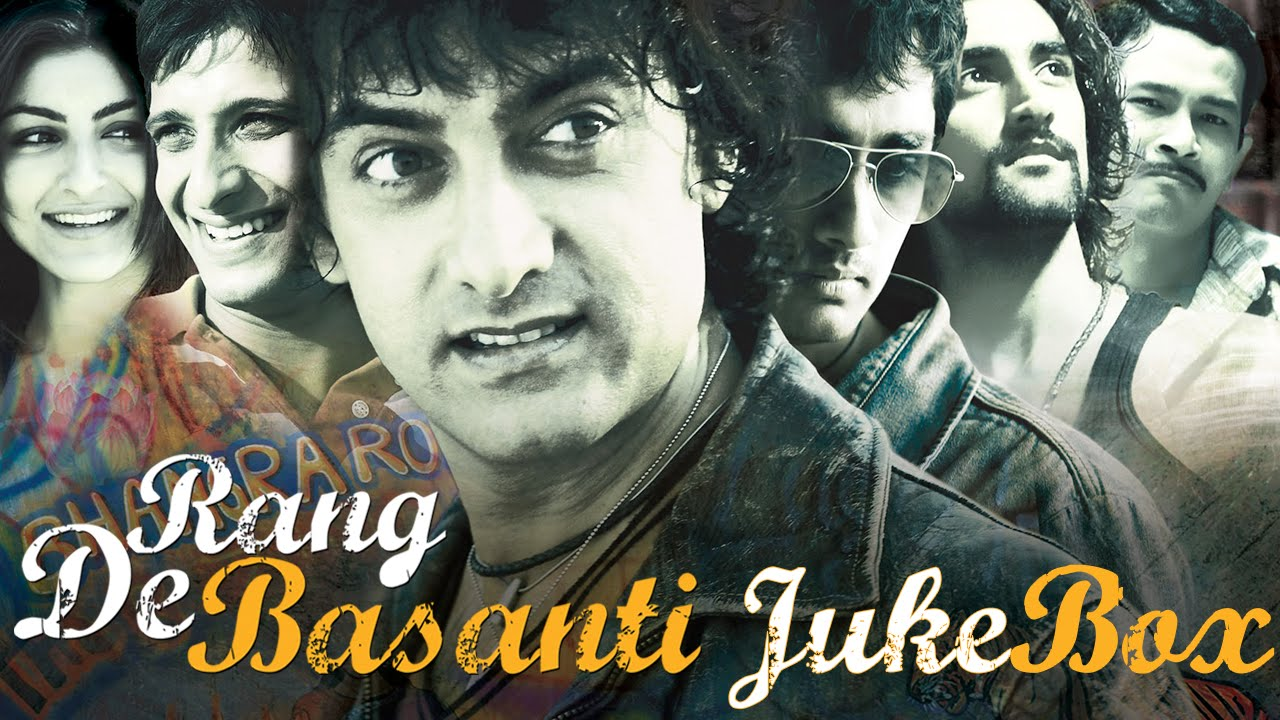
\includegraphics{pic.jpg}
\end{figure}
\end{document}
